Die gemessenen Umdrehungen lassen sich mit der Gleichung
\begin{align*}
  1 \text{Umdrehung} = \SI{0,1}{A}
\end{align*}
umrechnen. Aus der resultierenden Stromstärke kann das B-Feld berrechnet werden.
\begin{align*}
  B=\mu_0\frac{8}{\sqrt{125}}\frac{N\cdot I}{R}
\end{align*}
Die Errechnete Werte sind zusammen mit den dazugehörigen Frequenzen in der Tabelle \ref{tab.Tab1} einzusehen.
\begin{table}
  \centering
  \caption{In Abhängigkeit der eingestellten Frequenz aufgenommene Stromstärken durch die beiden Horizontalspulen. Aufgenommen wurden die Stromstärke an den Resonanzstellen für die beiden Isotope (1) und (2), mit dem gegebenen Maßen der Spulen wurde das horizontale Gesamtfeld aus den Stromstärken bestimmt.}
  \label{tab.Tab1}
    \begin{tabular}{c c c c c c c}
      \toprule
      Frequenz  & Stromstärke & Stromstärke & B-Feld 1 & Stromstärke & Stromstärke &  B-Feld 2\\
        & Horizontalspule & Sweep-Spule & & Horizontalspule & Sweep-Spule&\\
      kHz & A& A& $\mu$T & A& A& $\mu$T\\
      \midrule
      \midrule
      100     & 0,000  &  0,501 &  30,234  &  0,000 &  0,621 &  37,476 \\
      200     & 0,024  &  0,432 &  47,117  &  0,024 &  0,677 &  61,902 \\
      300     & 0,045  &  0,451 &  66,680  &  0,045 &  0,833 &  89,733 \\
      400     & 0,060  &  0,400 &  76,757  &  0,060 &  0,880 & 105,724 \\
      500     & 0,081  &  0,324 &  90,587  &  0,081 &  0,907 & 125,769 \\
      600     & 0,093  &  0,390 & 105,093  &  0,111 &  0,824 & 147,069 \\
      700     & 0,111  &  0,342 & 117,982  &  0,138 &  0,769 & 167,429 \\
      800     & 0,114  &  0,549 & 133,105  &  0,180 &  0,510 & 188,631 \\
      900     & 0,138  &  0,440 & 147,574  &  0,204 &  0,544 & 211,730 \\
      1000    & 0,144  &  0,617 & 163,518  &  0,234 &  0,503 & 235,565 \\
      \bottomrule
    \end{tabular}
\end{table}

\FloatBarrier
In der Graphik \ref{fig:Bf} sind die Werte graphisch dagestellt.
Es wird eine Ausgleichsrechnung der Form:
\begin{align*}
  B(f)=af+b
\end{align*}
durchgeführt.
\begin{figure}[h!]
  \centering
  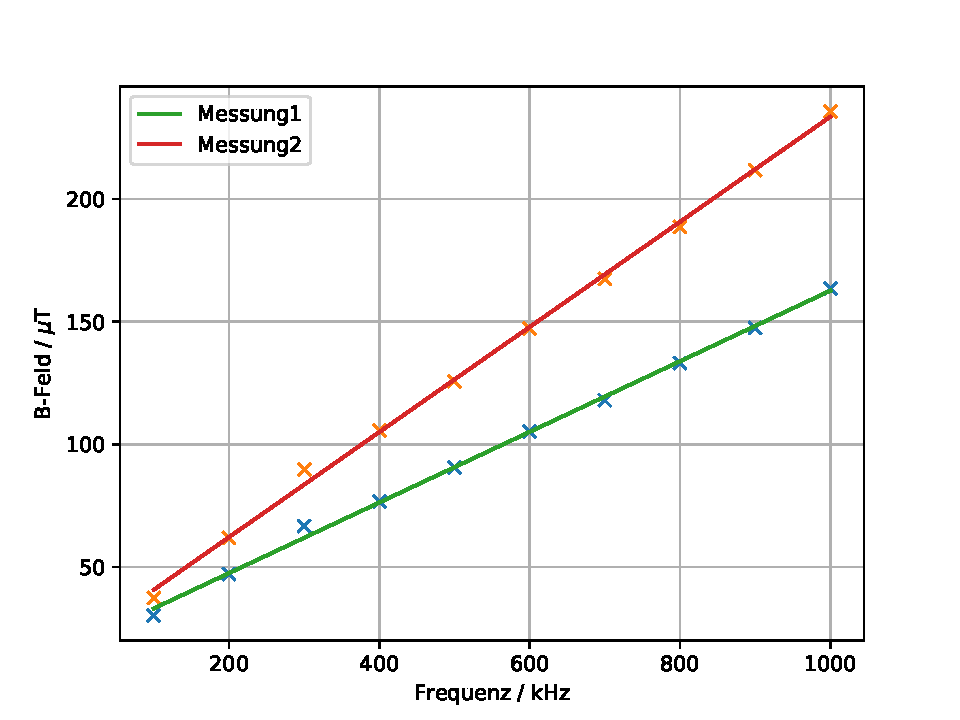
\includegraphics[width=0.8\textwidth]{B-Feld.pdf}
  \caption{Das für die Resonanzstelle benötigte Magnetfeld aufgetragen auf die Frequenz}
  \label{fig:Bf}
\end{figure}
\begin{align*}
  B1&\\
  a_1&=\SI{1.438\pm 0.023e-10}{\frac{T}{Hz}}\\
  b_1&=\SI{1.876\pm 0.144e-5}{T}
\end{align*}
\begin{align*}
  B2&\\
  a_2&=\SI{2.141\pm0.031e-10}{\frac{T}{Hz}}\\
  b_2&=\SI{1.935\pm0.190e-5}{T}
\end{align*}

Mit der Steigung kann wie folgt der Landesche $g_F$-Faktor bestimmt werden.
\begin{align*}
  g_F = \frac{h}{\mu_0\cdot a_i}
\end{align*}
Somit ergeben sich die Landeschen Faktoren zu:
\begin{align*}
  g_{F1} = 0.4967800215411603\\
  g_{F2} = 0.3337255596982711.
\end{align*}

\begin{align*}
  g_J = \frac{(g_s+1)\cdot J\cdot(J+1)+(g_s-1)\cdot[S\cdot (S+1)-L\cdot (L+1)]}{2\cdot J \cdot (J+1)}
\end{align*}
$g_s$ ist gegeben als
\begin{align*}
  g_s = 2,0023
\end{align*}
Die Quantenzalen in dem Versuch sind gegeben als
\begin{align*}
  S = \frac{1}{2}, L=0, J=\frac{1}{2}, F = I+J
\end{align*}
Durch einsezten ergibt sich, dass
\begin{align*}
  g_J=g_s
\end{align*}
ist.
Mit Hilfe der Formel
\begin{align*}
  I = \frac{1}{2}\left(\frac{g_J}{g_F}-1\right)
\end{align*}
ergeben sich Kernspinzahlen von
\begin{align*}
  I_1=1.515278305464324\\
  I_2=2.499920056783072
\end{align*}
